\documentclass[12pt]{article}
\usepackage{pdfpages}
\usepackage{eso-pic}
\usepackage{hyperref,url}
\usepackage{graphicx}
\graphicspath{{images/}}
\newcommand\tab[1][1cm]{\hspace*{#1}}

\begin{document}
\input{Titlu.tex}
\cleardoublepage

\newpage

\pagenumbering{arabic}
\setcounter{page}{1}
\setcounter{secnumdepth}{4}

\addtocontents{toc}{\protect\thispagestyle{empty}} % no page number on the table of contents page
\cleardoublepage

\section*{Lucrarea de laborator \#1}
\phantomsection

\section{Scopul lucrarii de laborator}
De a se invata utilizarea unui Version Control System si modul de setare a unui server.
\section{Obiective}
Studierea Version Control Systems (git).

\clearpage

\cleardoublepage

\section{Mersul lucrarii de laborator}

\subsection{Cerintele}

Initializarea unui nou repositoriu.\\
Configurarea VCS.\\
Commit, Push pe branch.\\
Folosirea fisierului .gitignore.\\
Revenire la versiunele anterioare.\\
Crearea branch-urilor noi.\\
Commit pe ambele branch-uri.\\
Merge la 2 branchuri.\\
Rezolvarea conflictelor.\\

\subsection{Analiza Lucrarii de laborator}
\tab Linkul la repozitoriu \textbf{https://github.com/Ernest96/MIDPS}\\
Sunt mai multe modalitati de a initializa un repozitoriu pe github.
Putem crea o mapa goala in care vom plasa gitul nostru prin intermediul comenzii \textbf{git init}.\\
\tab Urmatorul pas este crearea insusi a noului repozitoriu pe care il vom crea utilizind urmatoarea comanda
\textbf{curl -u 'USER' https.//api.github.com\\/user/repos -d '\{"name":"NUME"\}'}. Unde cuvintele scrise cu CAPS
se vor inlocui cu numele utilizatorului si numele repozitoriului.\\
\tab Dupa aceasta este necesar sa unim gitul nostru gol cu repozitoriul creat.
Vom folosi urmatoarea comanda \textbf{git remote add origin "Linkul la repo"}\\
\\
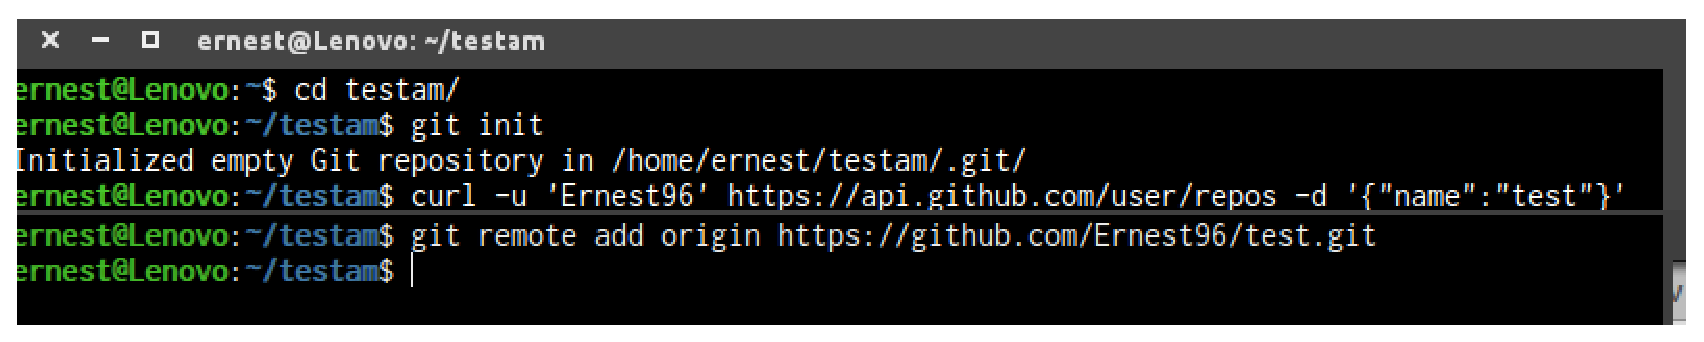
\includegraphics[width=\textwidth]{1.eps}
\clearpage
\tab O alta metoda de a crea un repozitoriu este cea online.
Pentru aceasta este nevoie sa deschidem pagina noastra pe github , sa alegem \textbf{repositories} si sa apasam butonul \textbf{new.}\\
\\

\includegraphics[width=\textwidth]{2.eps}
\\
\tab \textbf{Configurarea gitului} const in mai multe etape. La inceput vom configura numele si emailul.
Scrim urmatoarele comenzi:\\
\textbf{git config --global user.name "NUMELE"}\\
\textbf{git config --global user.email EMAIL}\\
\\
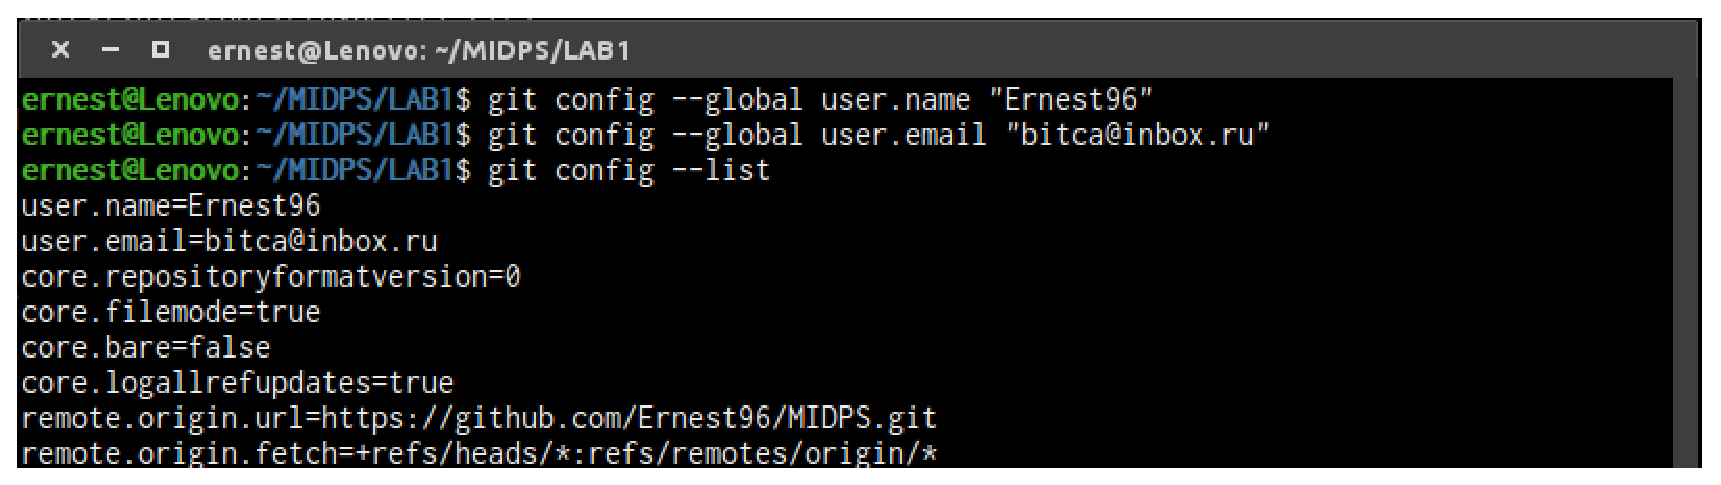
\includegraphics[width=\textwidth]{3.eps}
\\
\tab Urmatorul pas consta in generarea la cheia \textbf{SSH} (Secure Shell). Scriem in CLI \textbf{ssh-keygen},
iar cheia obtinuta o copiem in setarile noastre de pe git.
\tab Este de dorit sa initializam repozitoriul nostru cu un fisier \textbf{README.md} si un \textbf{.gitignore}. In fisierul
README.md vom adauga niste informatie pentru cei care se vor folosi de repozitoriu iar in fisierul .gitignore vom adauga
toate fisierele ce trebuiesc ignorate (adica sa nu fie incarcate).
\\
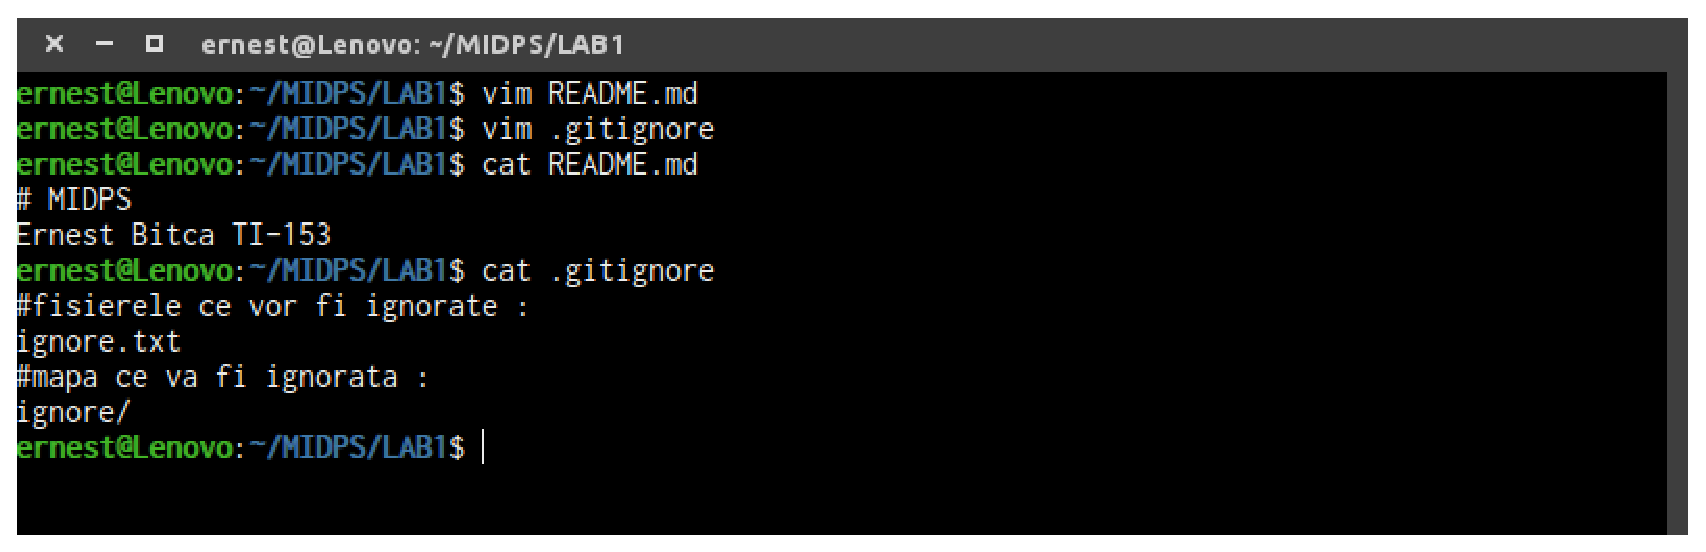
\includegraphics[width=\textwidth]{4.eps}
\\
\clearpage

\cleardoublepage
\tab Vom adauga fisierele noi create pe repozitoriul nostru. Pentru aceasta vom avea nevoie de
urmatoarele comenzi :\\
\textbf{git add *} - comanda indexeaza toate fisierele.\\
\textbf{git commit -m} - comanda face un snapshot la toate schimbarile noastre.\\
\textbf{git push origin master} - comanda incarca toate fisierele indexate pe git.


\tab Una dintre caracteristicele principale a unui \textbf{VCS} este faptul ca
ne permite sa revenim la o versiune mai veche. Aceasta poate fi efectuata cu ajutorul
comenzii \textbf{git reset --TYPE "codul comitului"}. Exista diferenta intre 
\textbf{--soft} si \textbf{--hard} , cind facem soft reset indexurile ramin neschimbate.
Iar in cazul cind facem hard reset , pierdem indexurile.
\\
\\
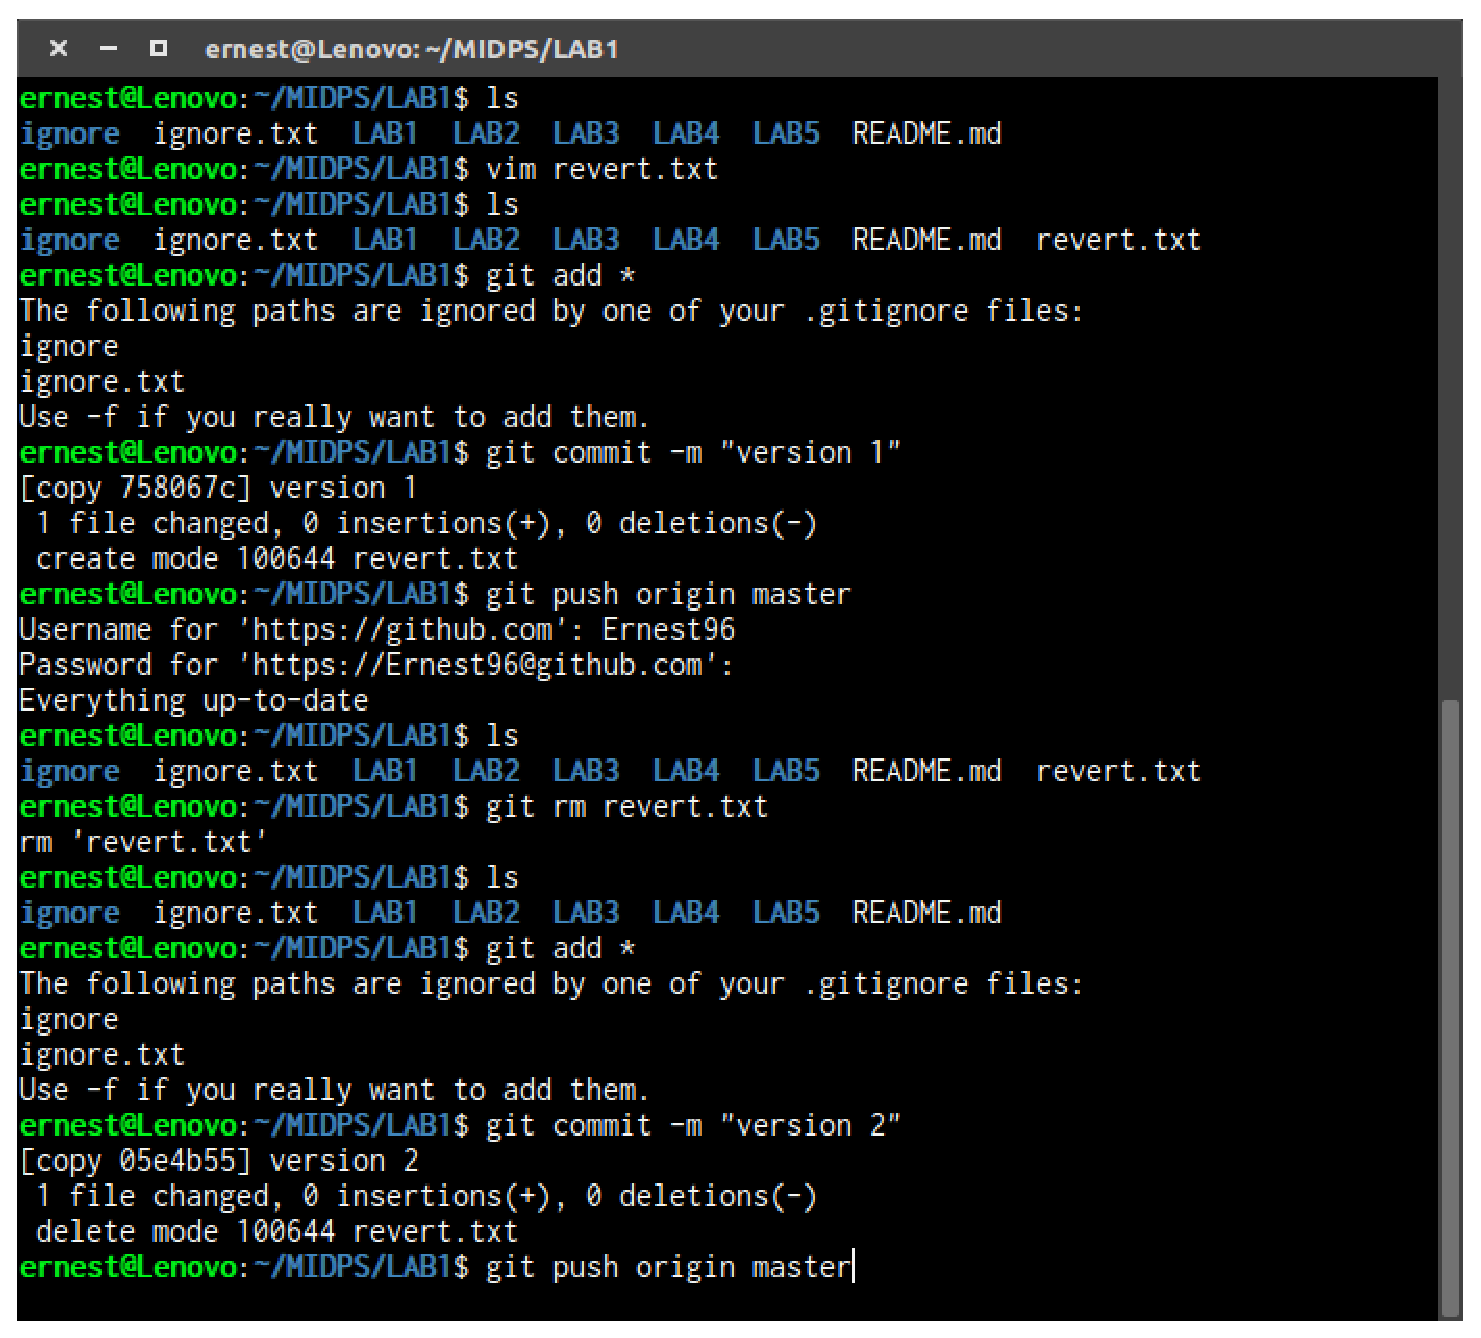
\includegraphics[width=\textwidth]{7.eps}
\\
\\
Dupa cum observam cind am facut commit, s-au ignorat fisierele incluse in .gitignore.
\clearpage
\tab Am creat un fisier nou revert.txt in versiunea 1. Dupa care l-am sters si am facut
commit la versiunea 2 in care am sters fisierul revert.txt dorim sa revenim la versiunea1. La inceput vom lansa comanda \textbf{git --log} care ne arata logul de commituri si
codul pentru fiecare commit. Vom avea nevoie de primele 7 cifre la commitul anterior.\\
\\
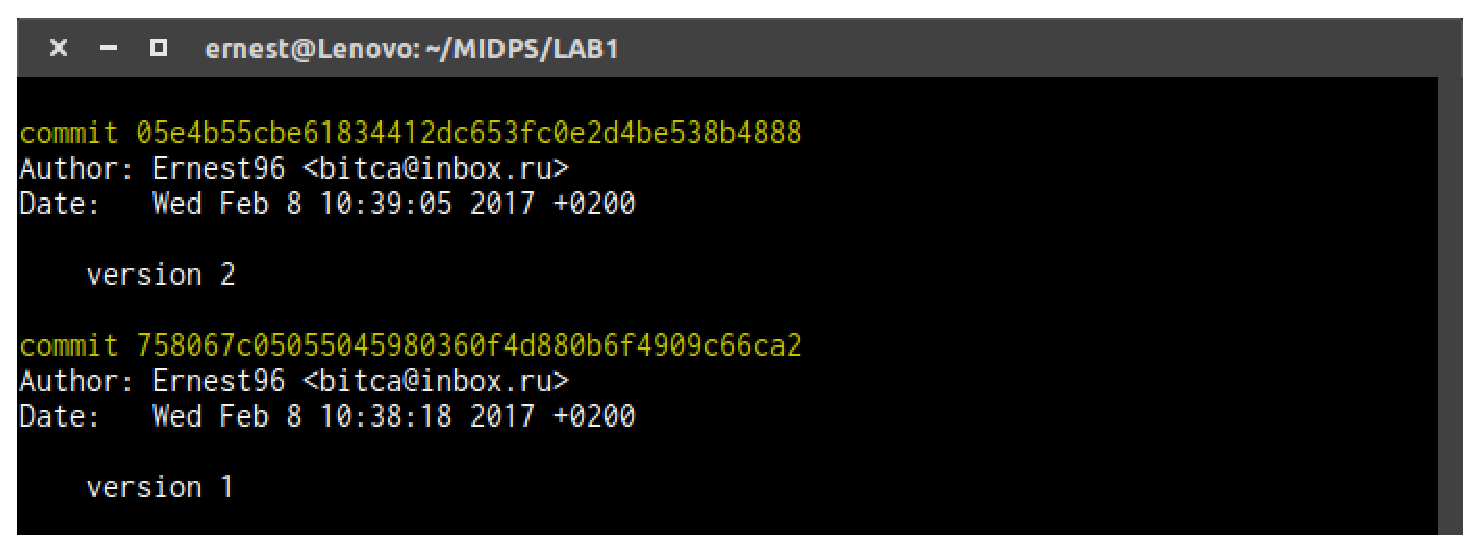
\includegraphics[width=\textwidth]{8.eps}\\
\\
Acum vom folosi comenzile descrise anterior.\\
\\
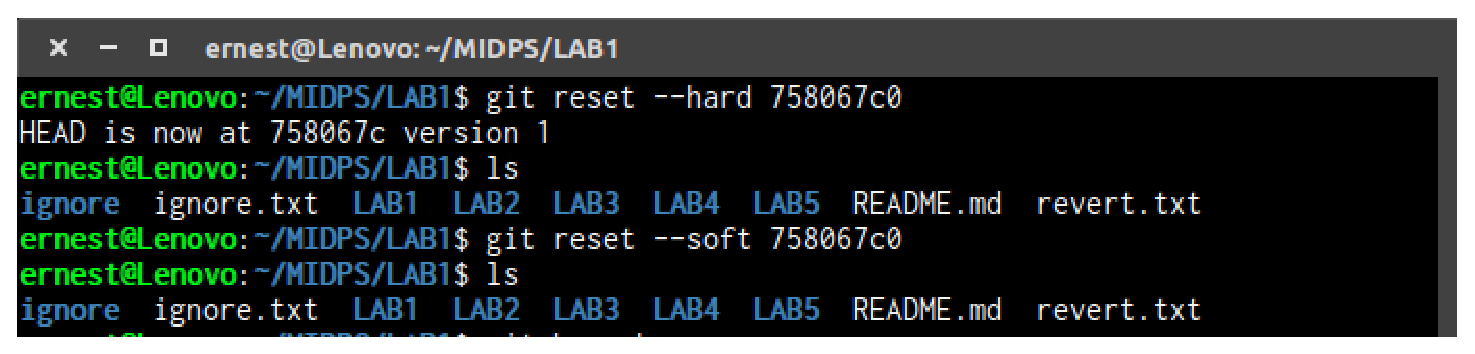
\includegraphics[width=\textwidth]{9.eps}\\

\cleardoublepage

~\\
\tab {VCS} ne permite sa avem mai multe \textbf{branchuri}.
Din traducere branch semnifica "creanga". Branchurile sunt foarte comod de folosit cind dorim sa lucram paralel la un proiect si apoi dorim sa unim toate modificarile.~\\
~\\
\textbf{git branch "name"} - creeaza un branch nou cu numele "name".~\\
\textbf{git branch} - vizualizarea branchurilor (* indica branchul curent).~\\
\textbf{git branch -d "nume"} - sterge branchul "nume".~\\
\textbf{git checkout -b "name"} - creeaza un branch nou cu numele "name" si
face switch la el.~\\
~\\
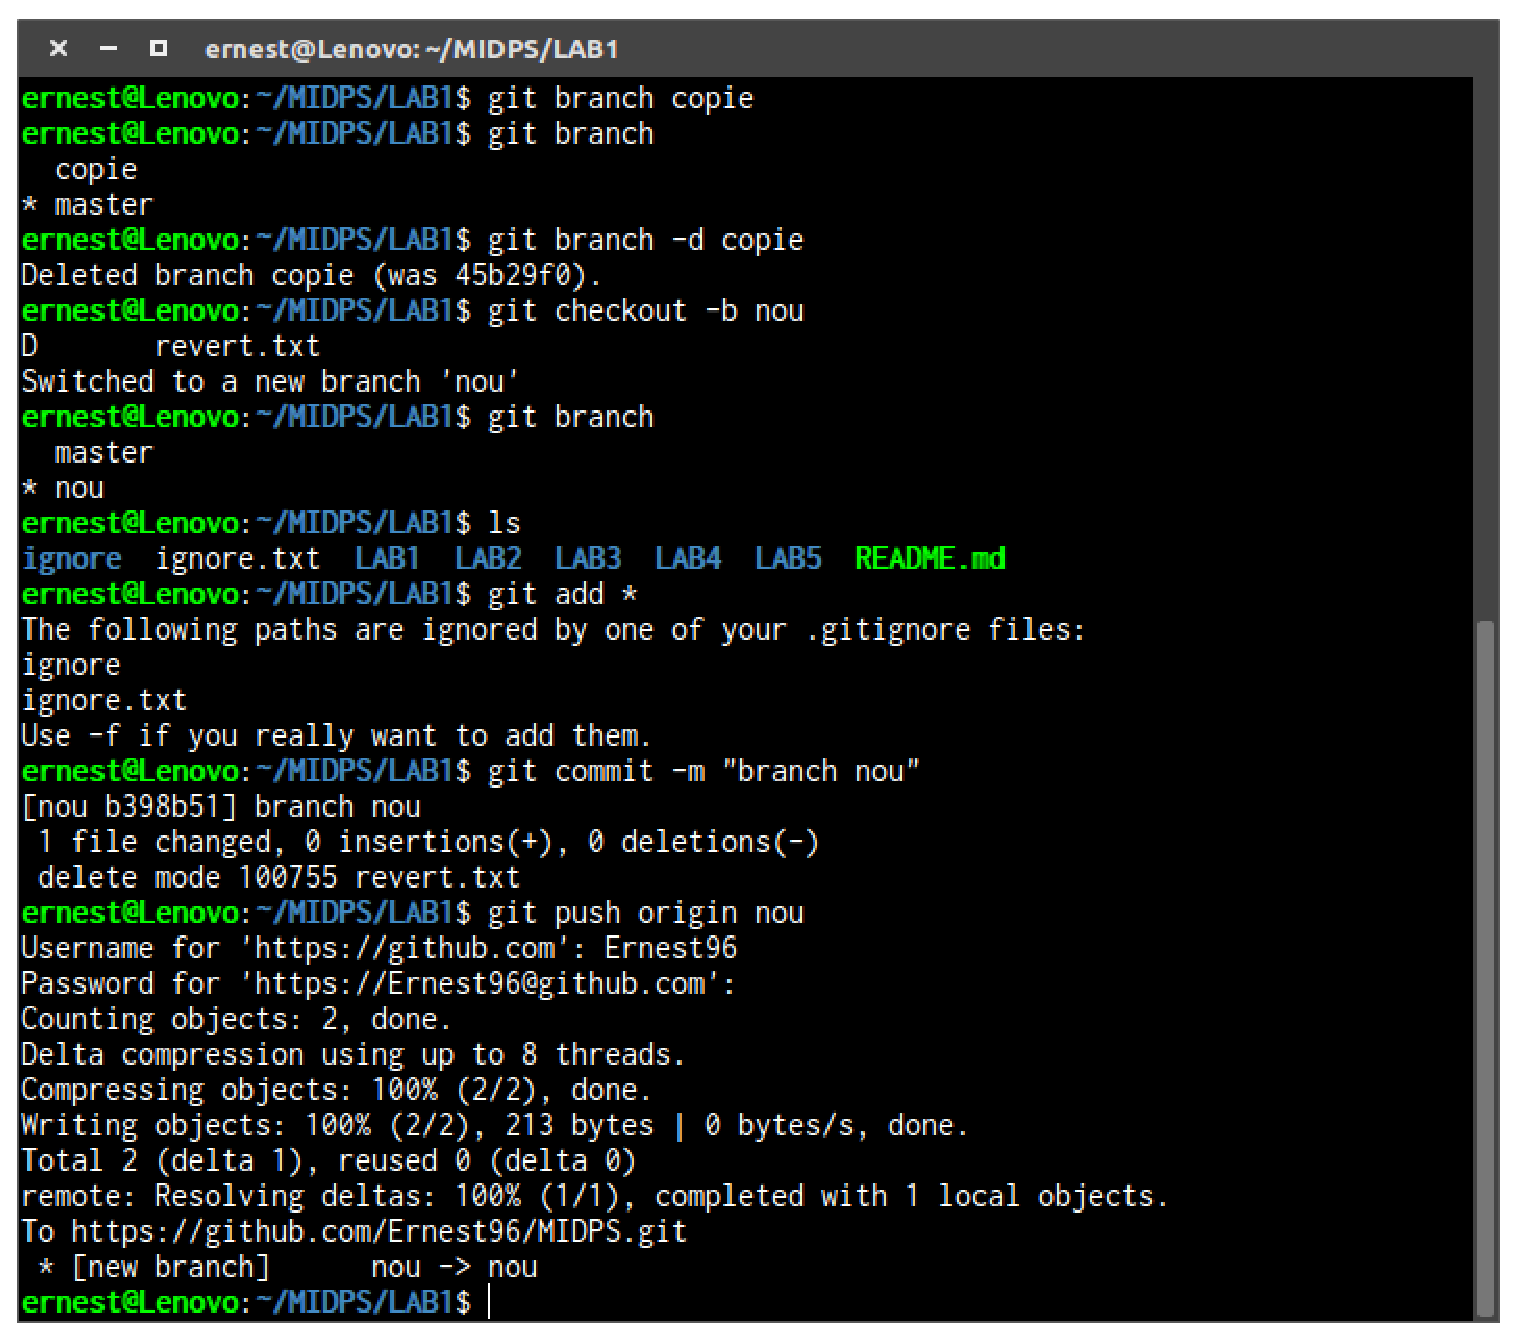
\includegraphics[width=\textwidth]{10.eps}~\\
\clearpage
~\\
\textbf{git checkout "nume"} - face switch la branchul "nume".~\\
\textbf{git branch -u upstream/name} - face track la branchul indicat din
branchul curent.~\\
\textbf{git branch -u upstream/name "nume" } - face track din branchul "nume"
la branchul indicat.~\\
\textbf{git branch --track "name" upstream/name} - creeaza branchul "name" si ii face track
la branchul indicat.~\\
\textbf{git branch --unset-usptream} - scoate trackingul la branchul in care ne
aflam.~\\
~\\
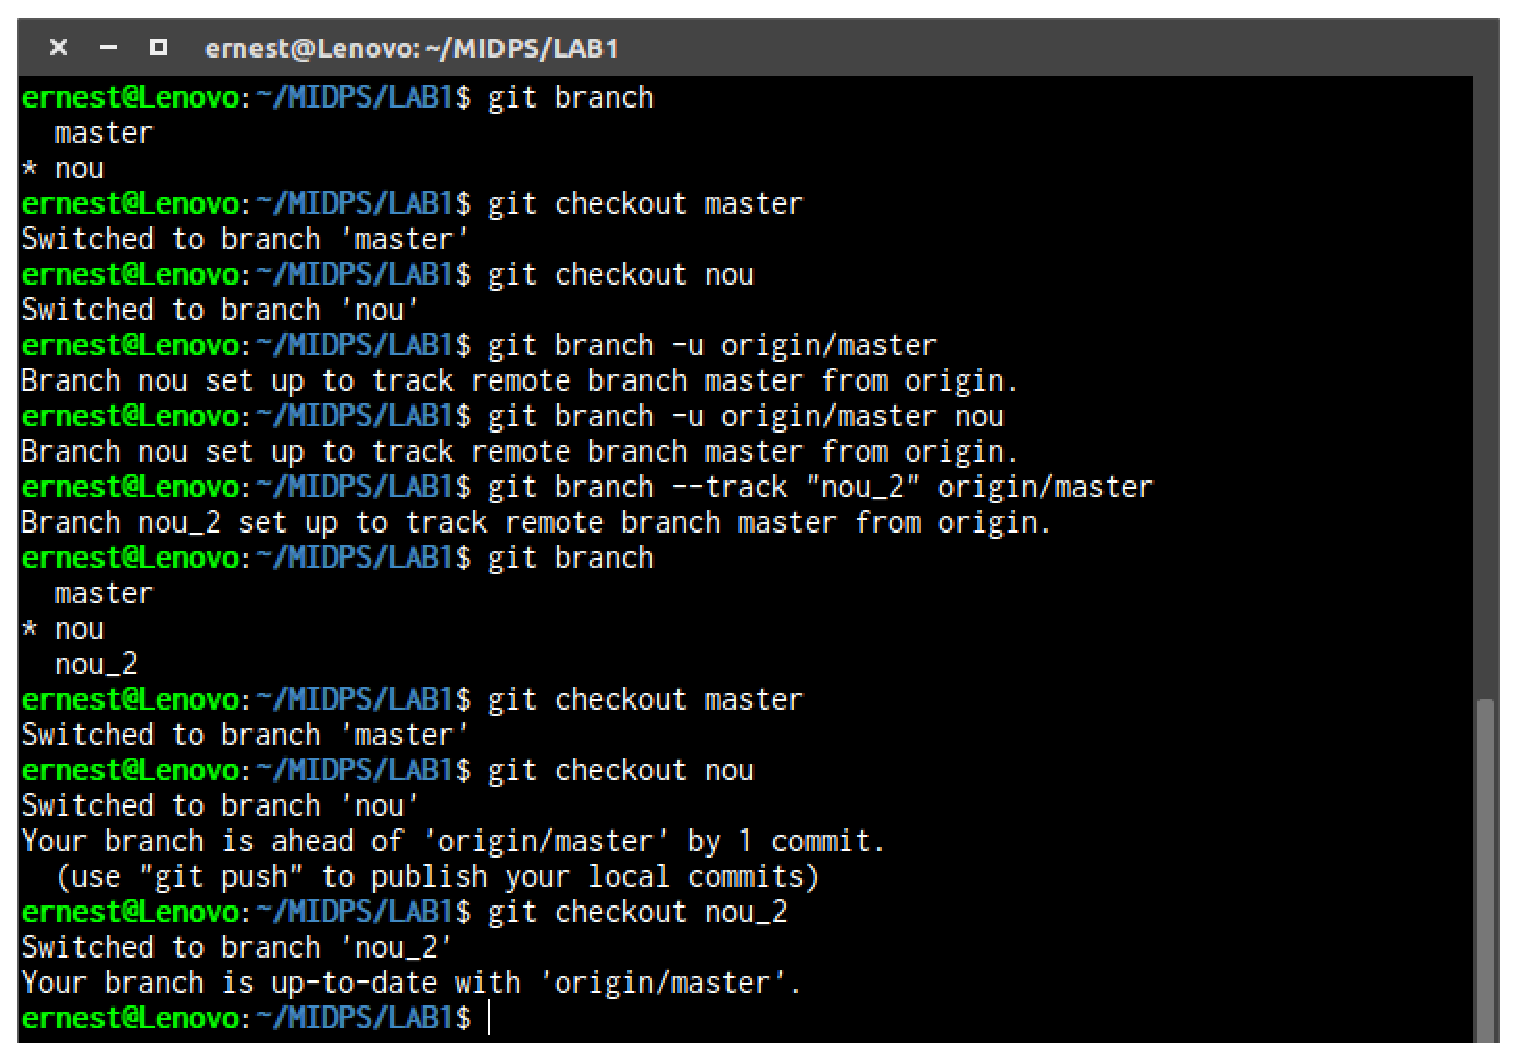
\includegraphics[width=\textwidth]{12.eps}~\\
~\\

\cleardoublepage

\tab Putem avea conflicte in cazul cind dorim sa facem merge la 2 branchuri si unele
rinduri sunt diferite. In asa caz ne vin in ajutor un mergetool. Drept mergetool am ales
\textbf{kdiff3}. Pentru a seta kdiff3 ca mergetool default folosim comanda : 
\textbf{git config --global merge.tool kdiff3}
~\\
\tab In continuare vom lucra cu 2 branchuri - "master" si "nou". Vom crea in fiecare
branch cite un fisier "tomerge" continutul caruia va fi diferit.\\
~\\
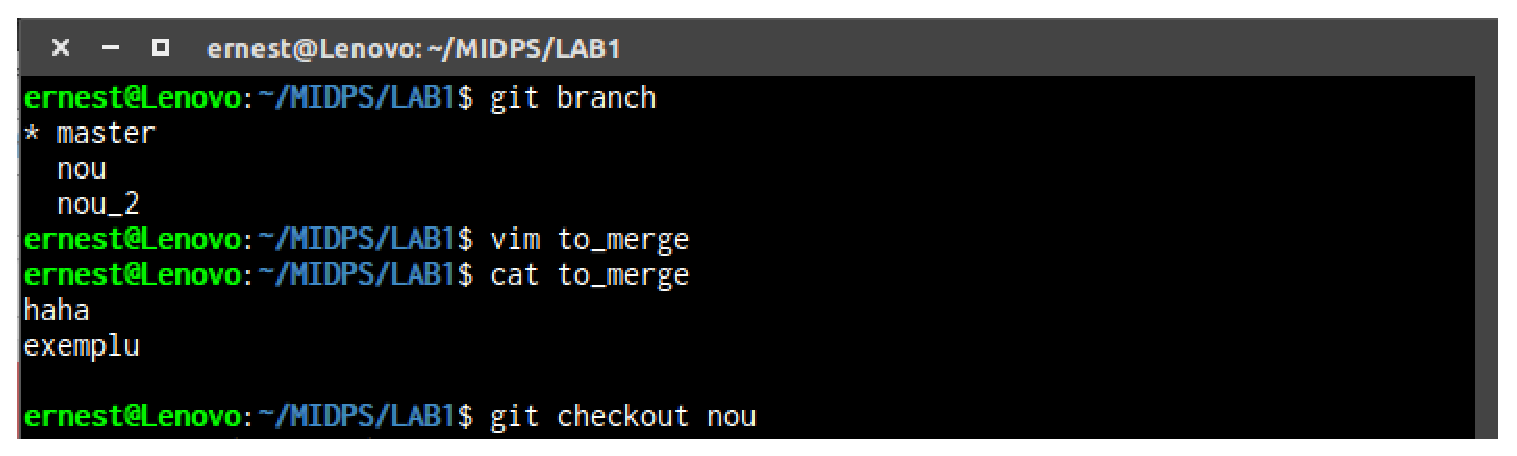
\includegraphics[width=\textwidth]{13.eps}\\
~\\
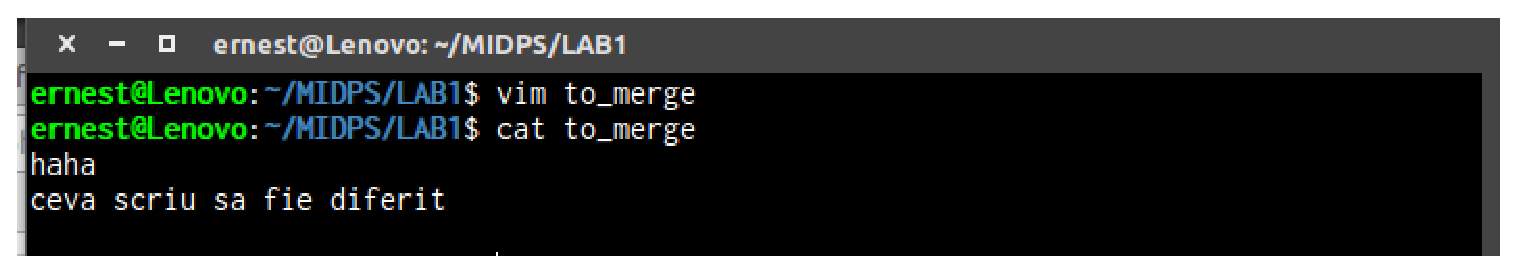
\includegraphics[width=\textwidth]{14.eps}\\
~\\
In continuare vom incerca sa facem merge si sa rezolvam acest conflict.\\
~\\
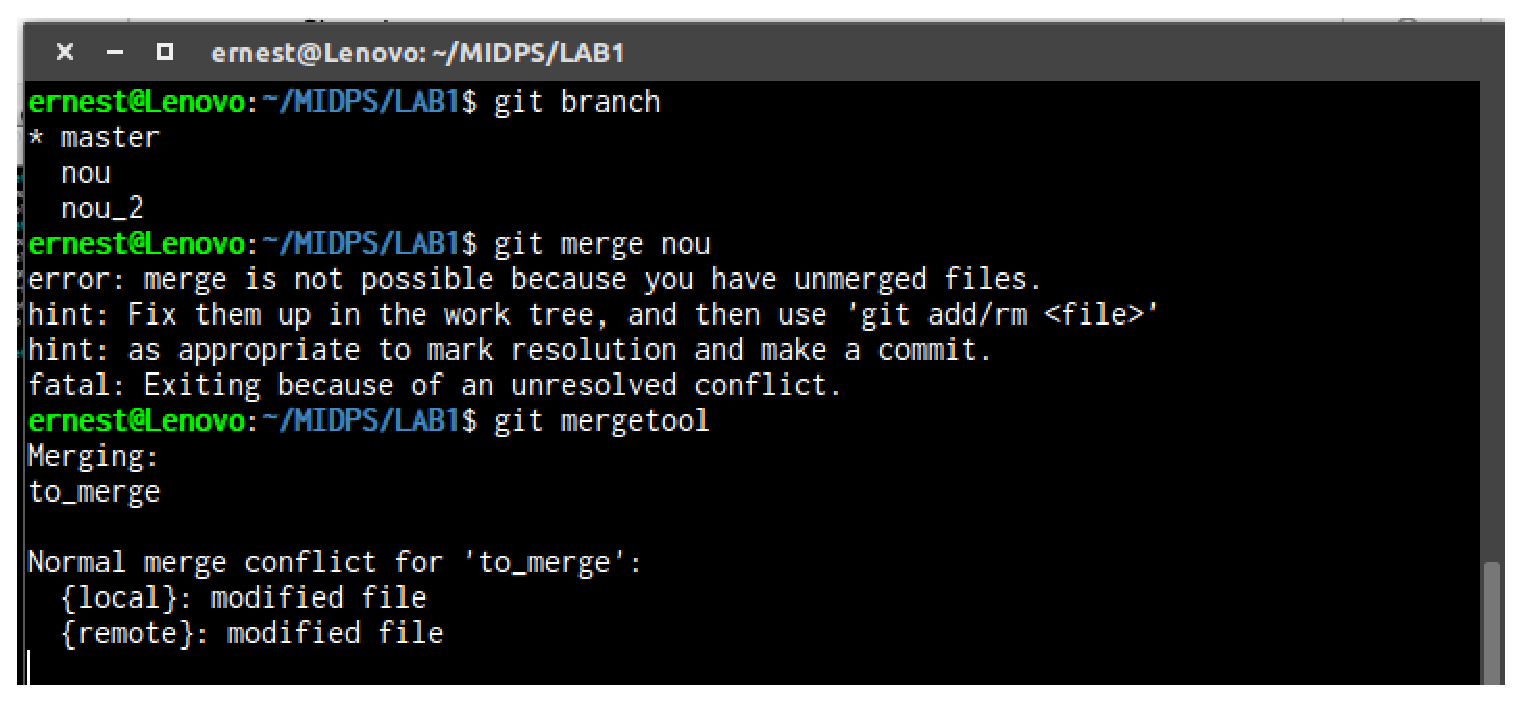
\includegraphics[width=\textwidth]{15.eps}\\
\clearpage
Dupa acest pas rezolvam conflictul cu ajutorul \textbf{kdiff3}. De exmplu eu 
am ales sa fac merge in felul urmator.\\
~\\
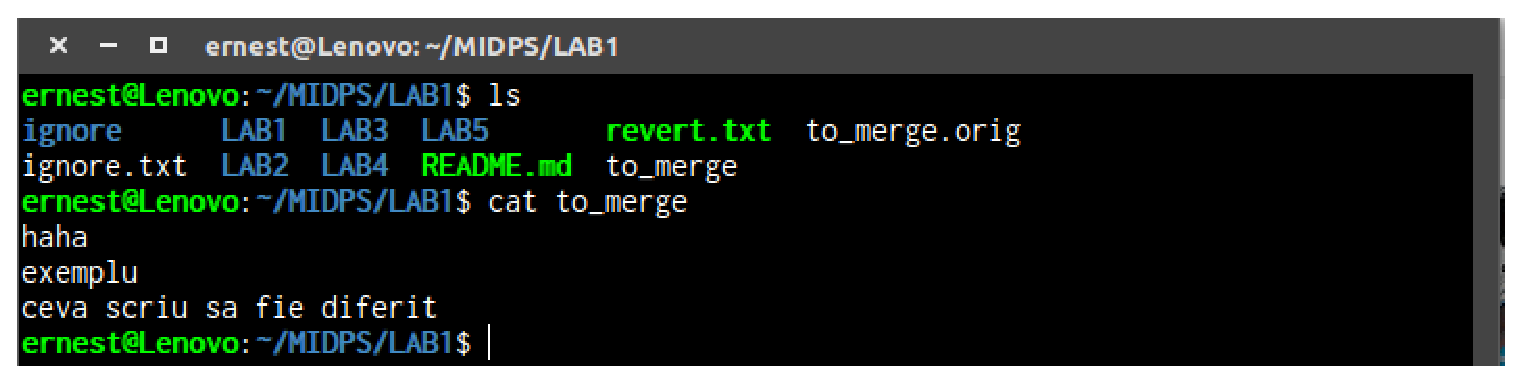
\includegraphics[width=\textwidth]{16.eps}\\
~\\
\textbf{Tagurile} sunt foarte comod de folosit si cu ajutorul lor putem face un track
eficient al versiunelor. Exemplu de tag.\\
\\
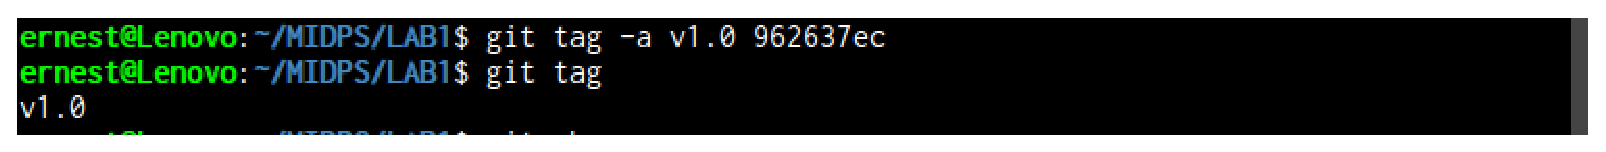
\includegraphics[width=\textwidth]{17.eps}\\
~\\
Dupa aceasta putem vedea usor o versiune taguita. Folosim comanda
\textbf{git show "tag"}\\
~\\
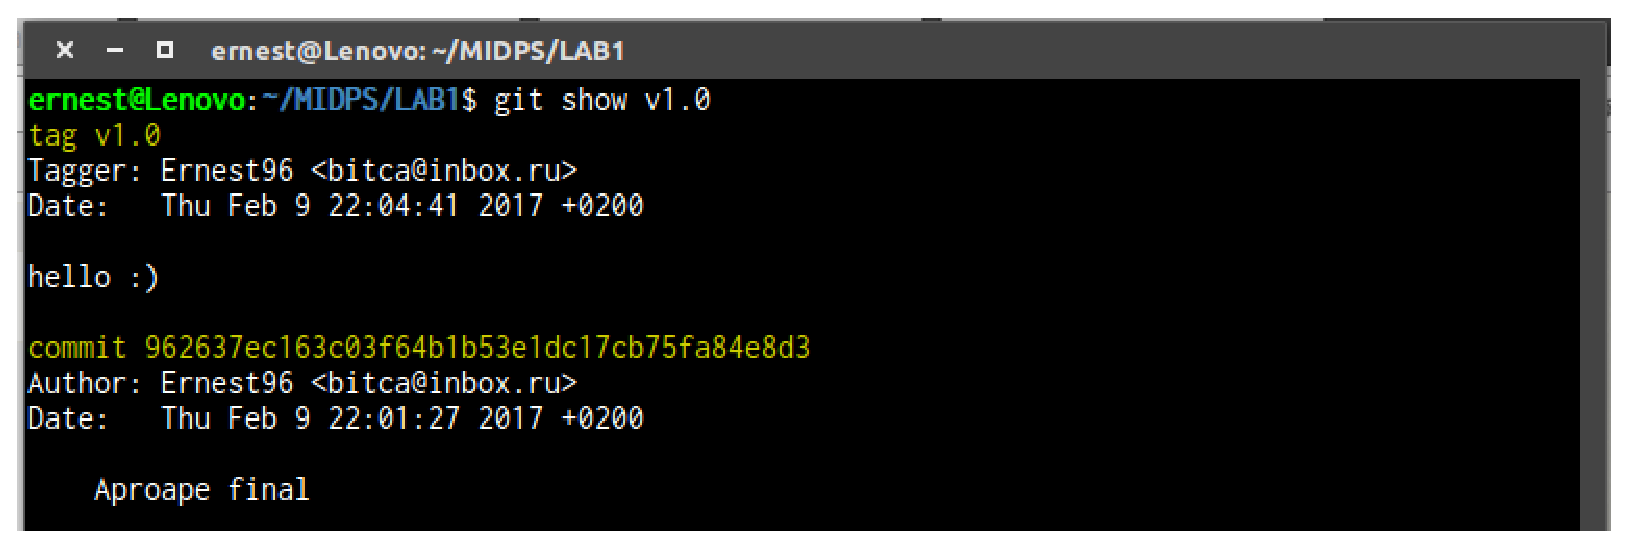
\includegraphics[width=\textwidth]{18.eps}\\
\clearpage

\cleardoublepage

\section{Concluzii}
\tab In lucrarea data am studiat lucrul cu \textbf{VCS}. Am luat cunostinta cu platforma
\textbf{github}. Toate lucrurile, comenzile le-am indeplinit in terminal pe Linux.
Sunt foarte multe plusuri in folosirea VCS. Fara el producerea produselor soft ar fi
foarte lenta si problematica. El ne permite lucrul paralel, menajarea versiunelor, 
revenire la versiuni anterioare. In lucrare am pus in practica majoritatea comenzilor
esentiale. Nu este prima mea experienta cu git-ul, insa mi-am imbunatatit nespus de mult
lucrul cu el. Am luat cunostinta cu branchurile, merge la branchuri si rezolvarea
conflictelor (utilizind kdiff3). Dupa parerea mea orice programator contemporan necesita
cunostinta unui VCS. El contribuie nu doar la dezvoltarea hard-skillurilor dar si a celor
soft.

\end{document}
